\chapter{Test Runner} \label{chap:TestRunner}
One of the primary goals of this application to give the lecturer a way to specify what constitutes a correct problem solution.
As previously mentioned in the \textbf{Use Cases} section of chapter \ref{chap:Specification}, a common approach to this is the use of test cases.

\section{Client-Server Interaction}
When a lecturer creates a new exercise, a modal prompts them to enter details about the exercise.
These details include the name of the exercise, instructions for the student, an optional code template to help the student get started, as well as test code.
This data is sent to the database where it is stored.
When a student opens an exercise, the data is then fetched from the database.
This is done by the client sending a request to the Next.js backend, which queries the database and returns both exercise and test data.

\begin{figure}[H]
    \centering
    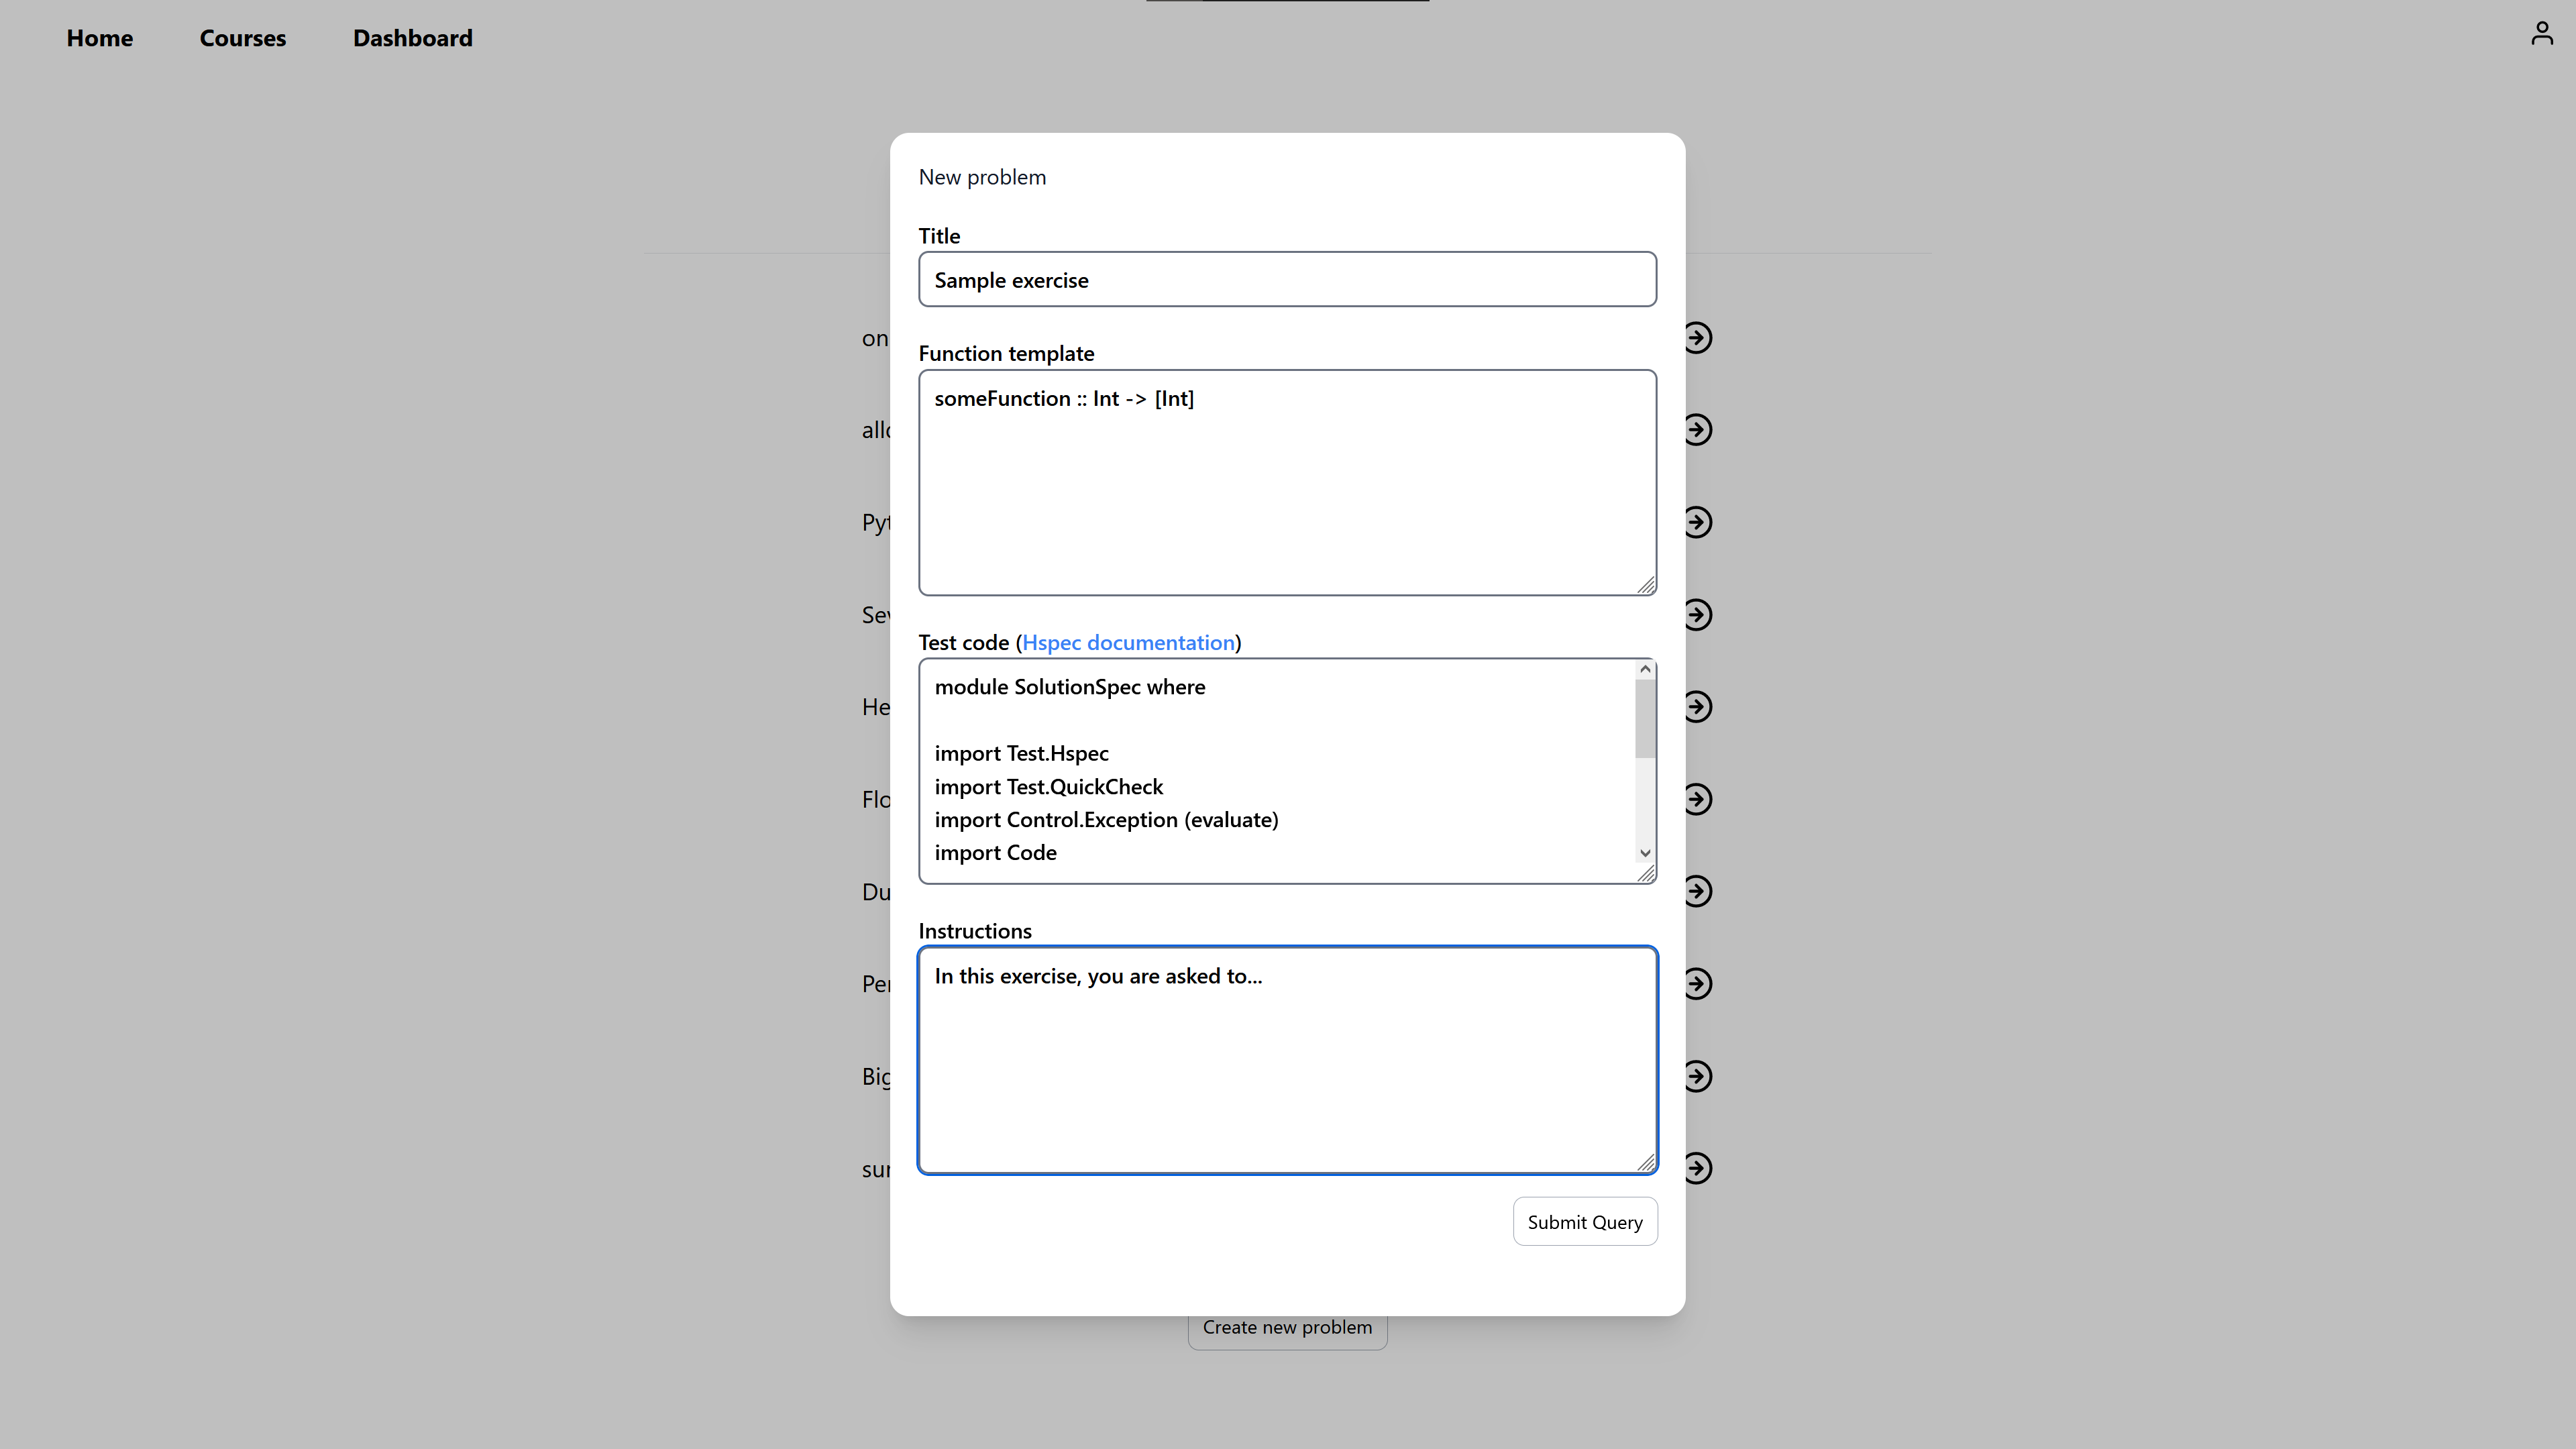
\includegraphics[scale=0.1]{create_exercise.png}
    \caption{Creating a new exercise as a lecturer}
    \label{fig:create_exercise}
\end{figure}

In the interest of reducing the number of database queries, the result of this request is cached on the client.
The client will eagerly request new data to stay up to date with instructions or test code updates.
We deemed that this short cache storage time is useful for when lecturers update test code during an exercise session.
This way, all students have the latest test code shortly after the update while still minimizing unnecessary queries.

When a user submits their exercise solution attempt, a mutation is sent to the Next.js backend.
In this request, the necessary code and test code is included.
One could argue that fetching the test code on the backend when processing this mutation would be more appropriate.
However, we want to eventually display the test code to the user so they may gain a better understanding of the solution requirements, although this will not be done in this iteration of the project.

To handle this mutation, the Next.js server requests the Test Runner to process the given solution and test code.
This process is described in section \ref{sec:test_runner_process} below.
The response of this request to the Test Runner is validated and stored as a submission in the database.
This allows users and lecturers to access previous submissions, which includes code and a value indicating whether the submission satisfied the exercise tests.

Lastly, the result is sent to the client and displayed on the page.

\begin{figure}[H]
	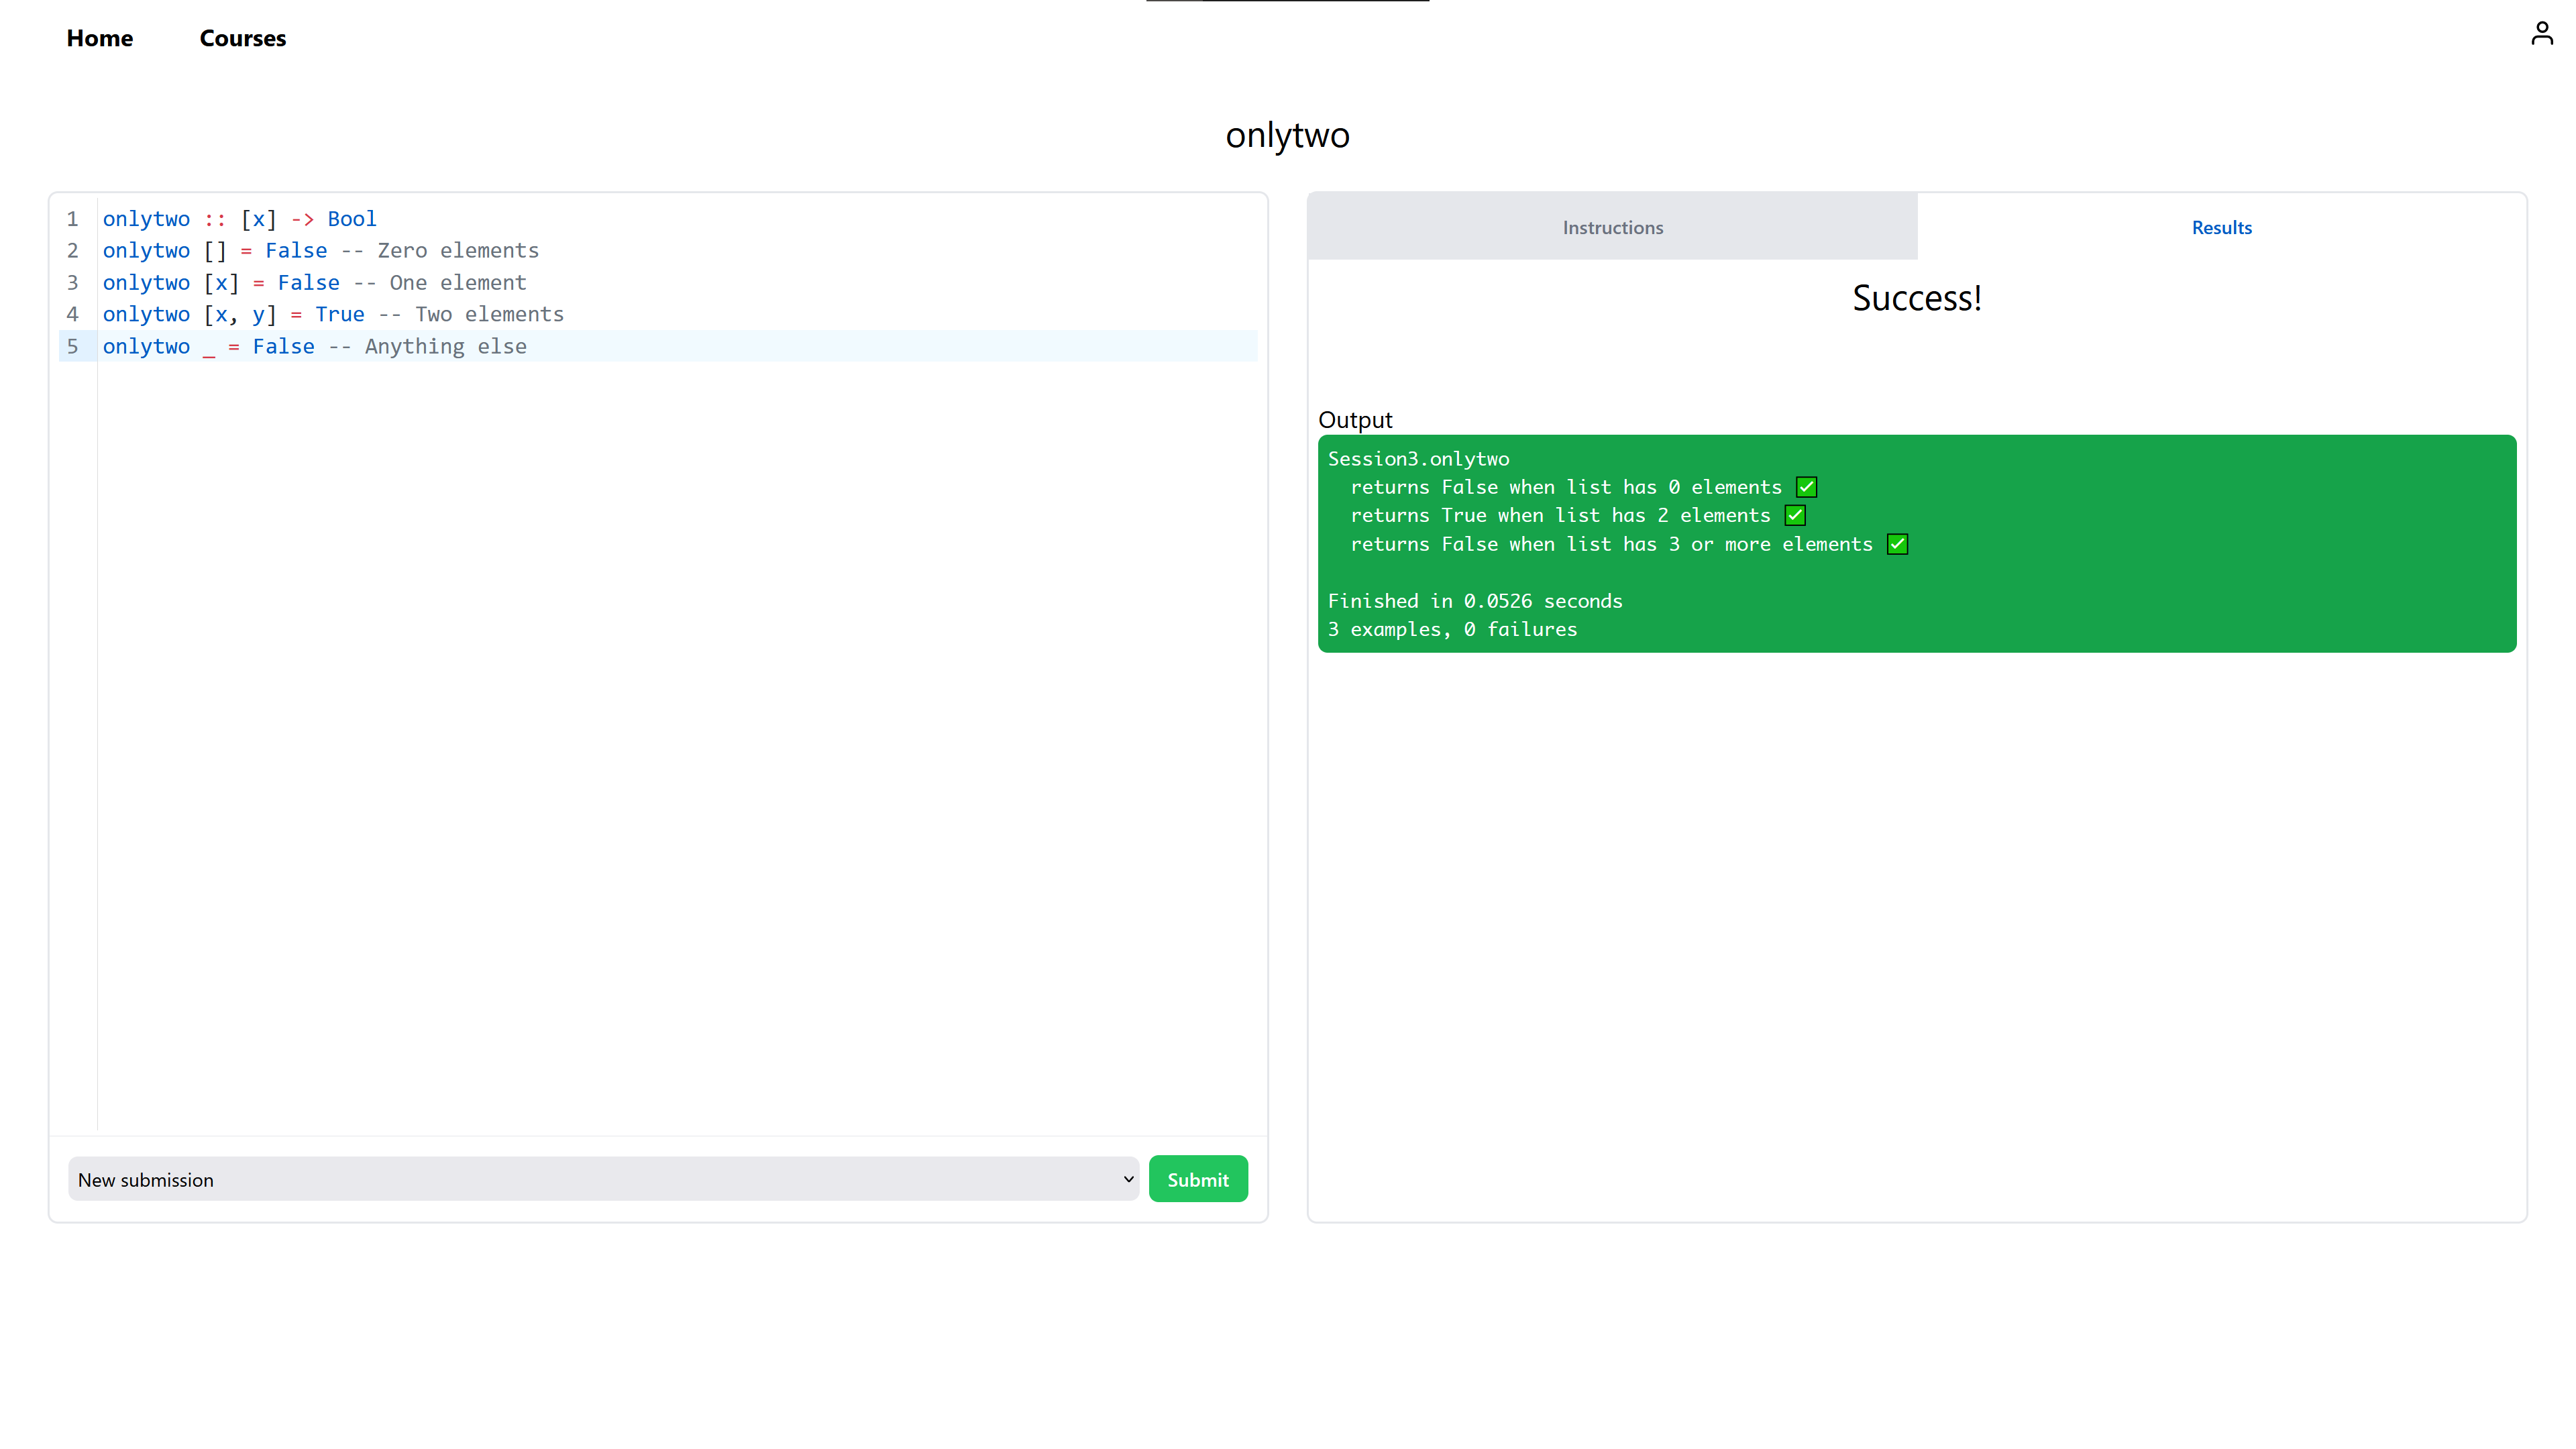
\includegraphics[scale=0.1]{exercise_success.png}
	\centering
	\caption{An example of a successful exercise submission}
	\label{fig:exercise_success}
\end{figure}

\begin{figure}[H]
	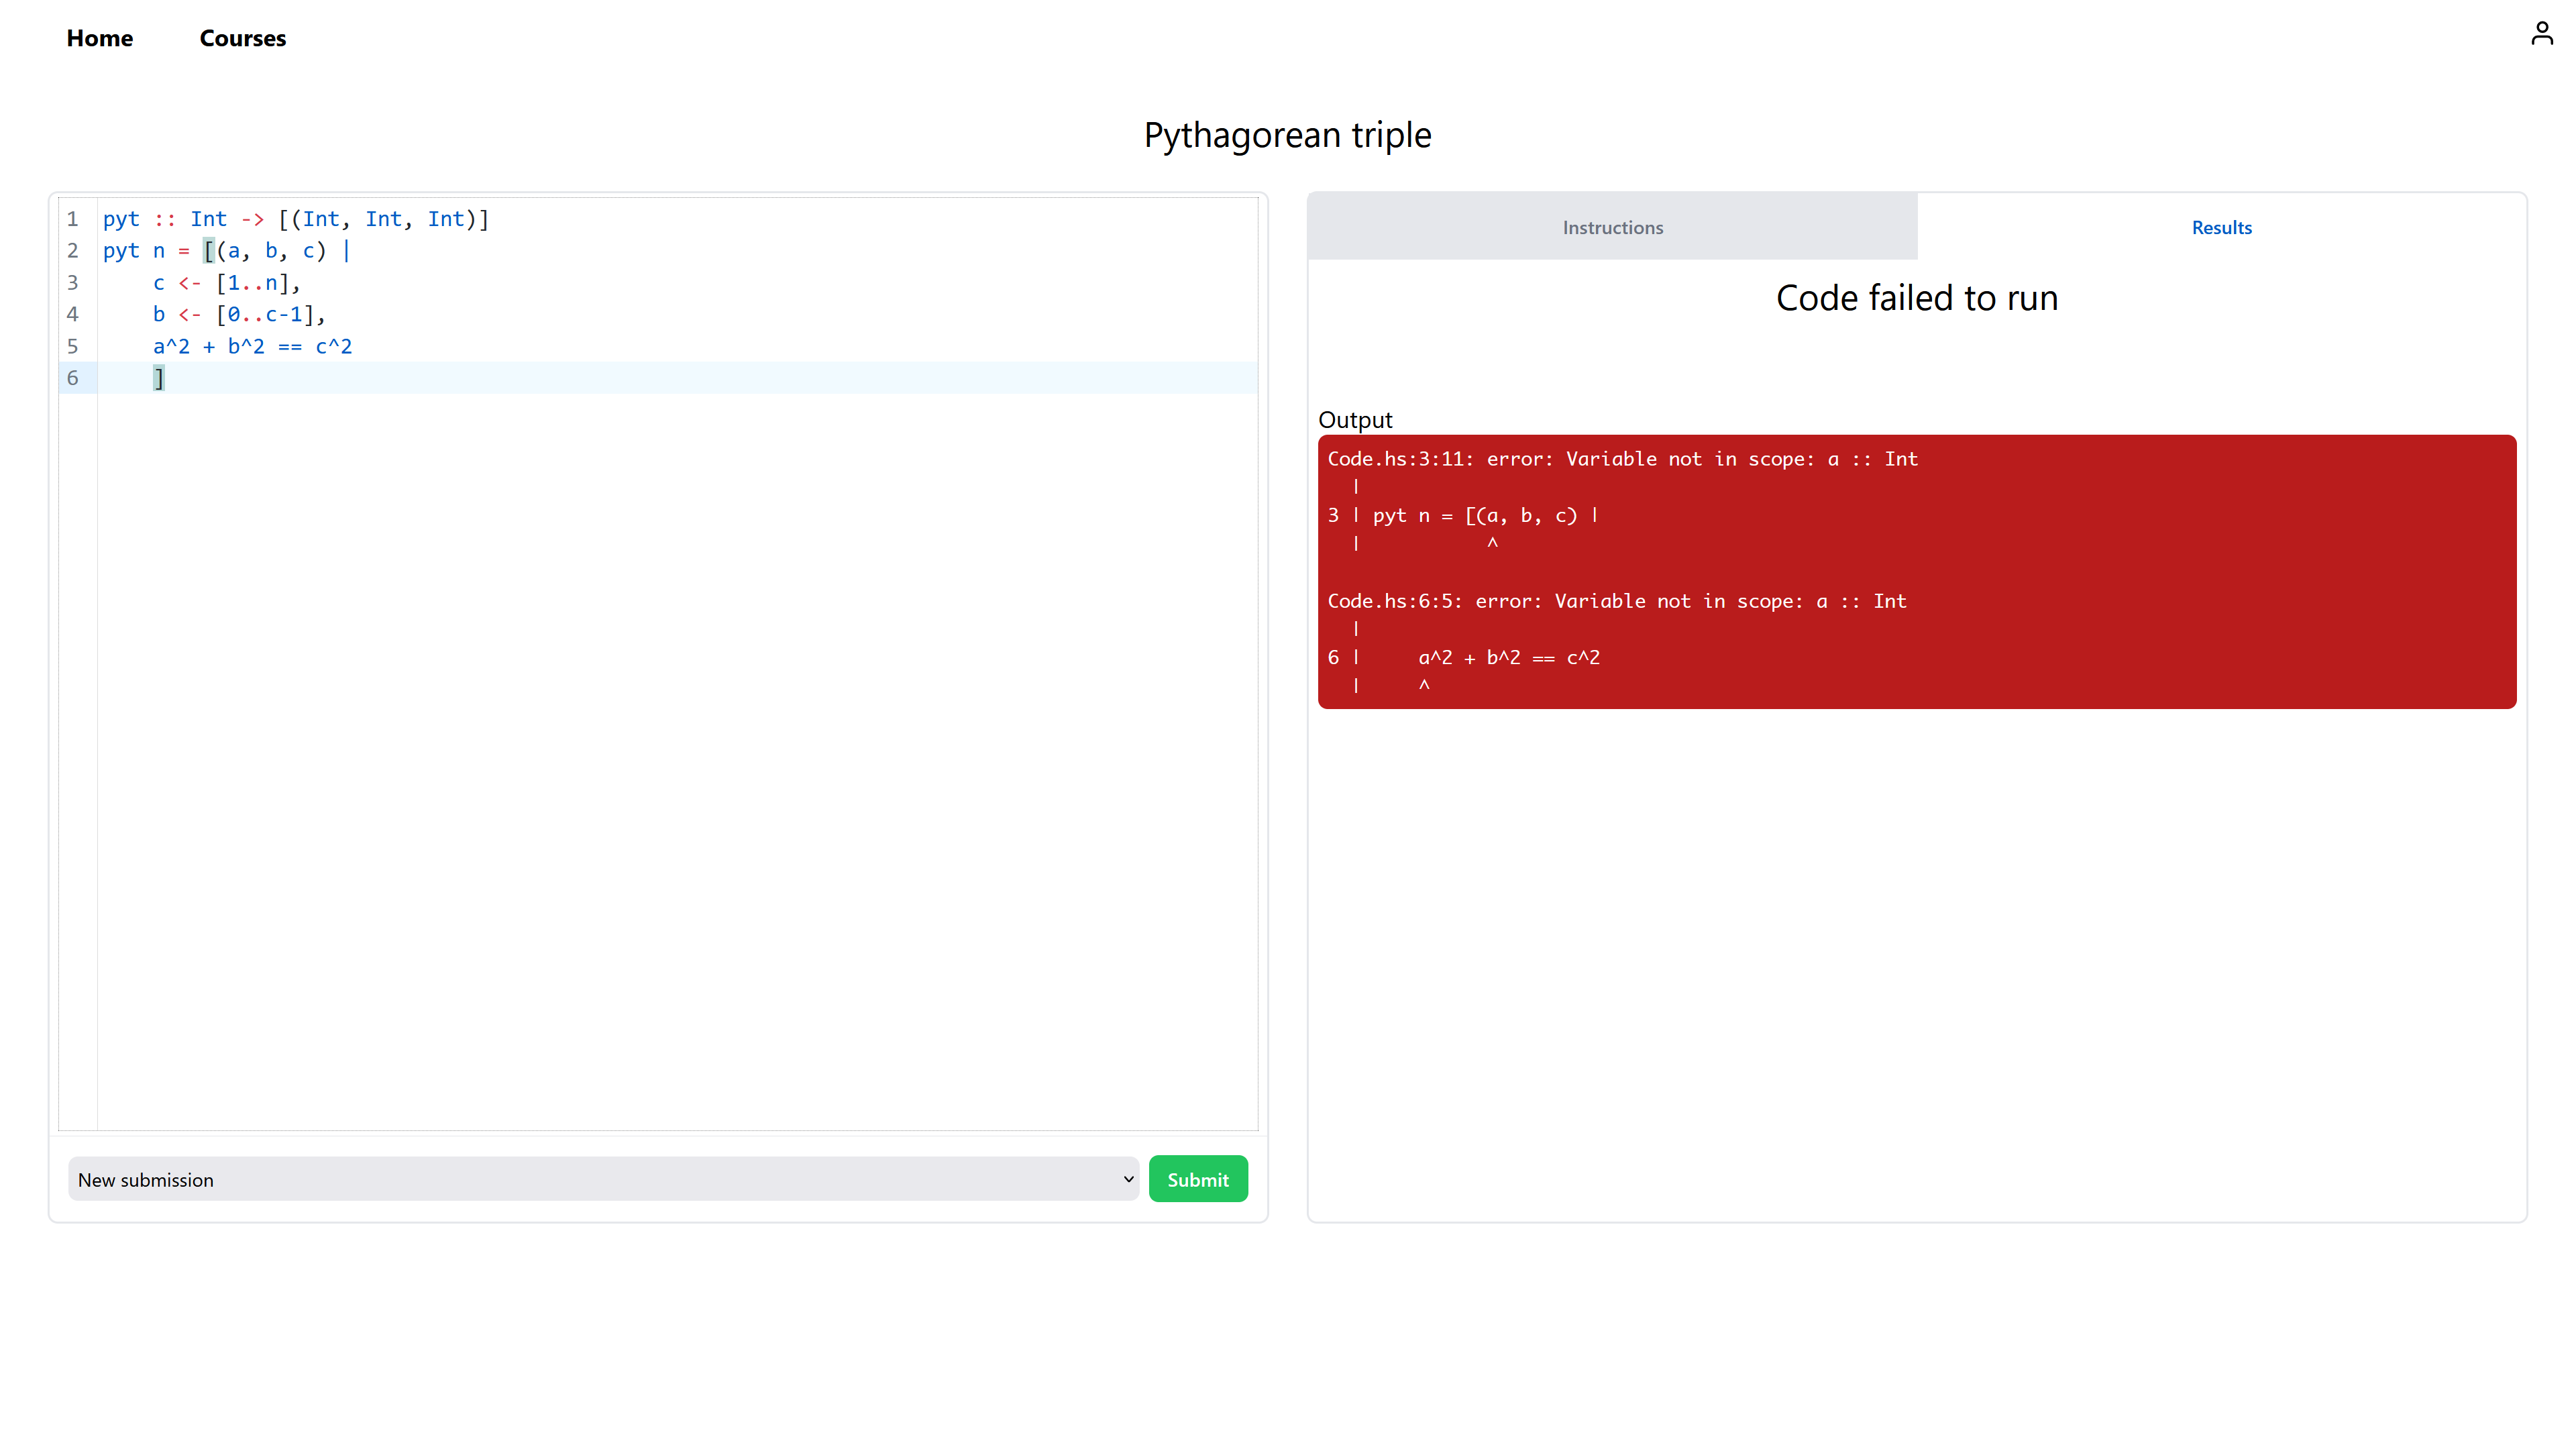
\includegraphics[scale=0.1]{exercise_fail.png}
	\centering
	\caption{An example of an unsuccessful exercise submission}
	\label{fig:exercise_fail}
\end{figure}

More images of the platform user interface can be seen in chapter \ref{chap:images} in the appendix.


\section{Test Runner Process} \label{sec:test_runner_process}
The Test Runner exposes an endpoint \texttt{/haskell/submit/}, which is used to post code submissions.
Originally, we used the Rust crate Rocket to implement this endpoint.
However, we eventually switched to using the axum crate instead, as it is developed and maintained by the same developers behind the Tokio package we make heavy use of for asynchronous programming and multithreading.
Furthermore, it was deemed easier to implement a shared state among endpoints by leveraging axum's \texttt{layer} feature.
We give an overview and a more technical explanation of how this was done in section \ref{sec:queue-system}.

When the Test Runner receives the request from Next.js, its singular goal is to run the tests against the code and send the result of this back as fast as possible.
In order to run the tests, we need to run the GHC interpeter on the test code, which, in turns, need access to the exercise submission code.
The GHC interpreter can be run from the command line with arguments specifying the path Haskell file to run.
In other words, the Test Runner needs to write the user submission and corresponding test code to a file.
However, if more users were to make a submission at the same time, the content of the file could potentially be overwritten while the GHC interpreter is running the tests.

To address this, we generate a new directory with a unique name for each submission.
Then, the user submission is written to two  \texttt{.hs} files inside this directory - a \texttt{code.hs} file containing the exercise submission, and a \texttt{test.hs} file containing the corresponding tests.
This way, we can pass the path to this isolated directory to the GHC interpreter process as an argument.
Once the tests have been run, the directory and its contents are deleted again.
The \texttt{stdout} of the process is then read to determine whether the tests succeeded or not.
Finally, the interpreter output and the test success flag is packaged into a JSON object and sent back to the client.

Sequentially starting a new \texttt{runhaskell} process for each request was identified as a major bottleneck during testing, which will be described in detail in chapter \ref{chap:Benchmarking}.
In order to address this, we started by refactoring the code base to allow running several instances of the GHC interpreter process at the same time.
However, despite this running faster for a small number of clients, this approach in itself is not sufficiently stable:
If multiple clients were to post a code submission at the same time, the Test Runner will start a new process for each request.
Given a large enough number of requests, this would crash the Test Runner web server.
Therefore, we needed a way to limit the number of running GHC interpreter processes while at the same time storing subsequent requests for future processing.